\documentclass{article}
\usepackage[utf8]{inputenc} % Handle UTF-8 encoding
\usepackage{amsmath, amssymb, tikz, geometry, multicol}
\usetikzlibrary{calc}
\geometry{margin=0.15in}
\tolerance=1000

\begin{document}

% Start of the document with two columns
\begin{multicols}{2}

% Left Column: Triangles
\section*{Trigonometry with Triangles}

\subsection*{Right Triangle Definitions}
\begin{center}
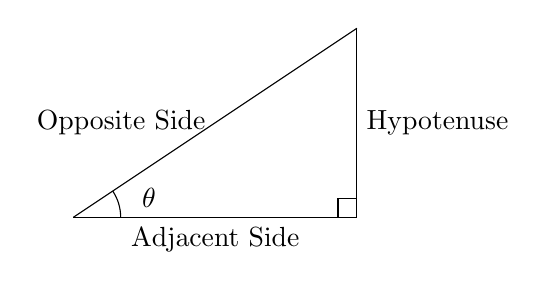
\begin{tikzpicture}[scale=1.2]
    \coordinate (A) at (0,0);
    \coordinate (B) at (3,0);
    \coordinate (C) at (3,2);
    \draw (A) -- node[below] {Adjacent Side} (B);
    \draw (A) -- node[left] {Opposite Side} (C);
    \draw (B) -- node[right] {Hypotenuse} (C);
    \draw (A) ++(0.5,0) arc (0:33.69:0.5cm);
    \node at (0.8,0.2) {\(\theta\)};
    % Right angle symbol
    \draw (B) ++(-0.2,0) -- ++(0,0.2) -- ++(0.2,0);
\end{tikzpicture}
\end{center}
\[
\sin \theta = \dfrac{\text{Opposite}}{\text{Hypotenuse}}, \quad
\cos \theta = \dfrac{\text{Adjacent}}{\text{Hypotenuse}}, \quad
\tan \theta = \dfrac{\text{Opposite}}{\text{Adjacent}}
\]
\[
\tan \theta = \dfrac{\sin \theta}{\cos \theta}, \quad
\csc \theta = \dfrac{1}{\sin \theta}, \quad
\sec \theta = \dfrac{1}{\cos \theta}, \quad
\cot \theta = \dfrac{1}{\tan \theta}
\]

\subsection*{Reference Angles}

A reference angle is the acute angle (\(<90^\circ\)) formed by the terminal side of an angle and the horizontal axis.

\begin{center}
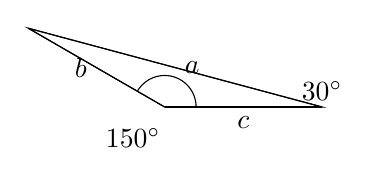
\begin{tikzpicture}[scale=2]
    % Define points
    \coordinate (A) at (0,0); % Point A (origin)
    \coordinate (B) at (1,0); % Point B on the positive x-axis
    % Point C calculated to form a 150-degree angle at A
    \coordinate (C) at ({cos(150)}, {sin(150)}); % Coordinates using degrees

    % Draw triangle
    \draw (A) -- (B) -- (C) -- cycle;

    % Label sides
    \draw (A) -- node[below]{$c$} (B);
    \draw (B) -- node[right]{$a$} (C);
    \draw (C) -- node[left]{$b$} (A);

    % Mark angle at A (150 degrees)
    \draw (A) ++(0.2,0) arc (0:150:0.2cm);

    % Move the 150-degree label outside the triangle towards the bottom left
    \node at ($(A)+(-0.2,-0.2)$) {\(150^\circ\)};

    \node at ($(A)+(1,0.1)$) {\(30^\circ\)};
\end{tikzpicture}
\end{center}

In this triangle, angle \( A \) is \(150^\circ\), and the reference angle \( \theta_{\text{ref}} \) is:

\[
\theta_{\text{ref}} = 180^\circ - 150^\circ = 30^\circ
\]


\textbf{Example:}  Find the reference angle for \( \theta = 150^\circ \).

\[
\theta_{\text{ref}} = 180^\circ - 150^\circ = 30^\circ
\]

So, the reference angle is \(30^\circ\).

When calculating trigonometric functions for obtuse angles, use the reference angle and adjust the sign based on the quadrant.


\textbf{Example:}  Find \(\sin 150^\circ\).

\[
\sin 150^\circ = \sin (180^\circ - 30^\circ) = \sin 30^\circ = \dfrac{1}{2}
\]

Since \(150^\circ\) is in Quadrant II, (sin+), \(\sin 150^\circ = \dfrac{1}{2}\).

\textbf{Example:}  Find \(\cos 150^\circ\).

\[
\cos 150^\circ = -\cos 30^\circ = -\dfrac{\sqrt{3}}{2}
\]

Since \(150^\circ\) is in Quadrant II, (cos-), \(\cos 150^\circ = -\dfrac{\sqrt{3}}{2}\).

\subsection*{Signs of Trigonometric Functions}
\begin{center}
\begin{tabular}{|c|c|}
\hline
Quadrant & Positive Functions \\
\hline
I & \(\sin\), \(\cos\), \(\tan\) \\
II & \(\sin\) \\
III & \(\tan\) \\
IV & \(\cos\) \\
\hline
\end{tabular}
\end{center}

\subsection*{Pythagorean Identity}
\[
\sin^2 \theta + \cos^2 \theta = 1
\]
\textbf{Example:} If \( \sin \theta = \dfrac{3}{5} \), then:
\[
\cos \theta = \sqrt{1 - \left( \dfrac{3}{5} \right)^2} = \dfrac{4}{5}
\]

\subsection*{Law of Sines}
\begin{center}
\begin{tikzpicture}[scale=1.2]
    \coordinate (A) at (0,0);
    \coordinate (B) at (3,0);
    \coordinate (C) at (1.5,2.5);
    \draw (A) -- node[below] {$c$} (B) -- node[right] {$a$} (C) -- node[left] {$b$} (A);
    \node[below left] at (A) {$A$};
    \node[below right] at (B) {$B$};
    \node[above] at (C) {$C$};
\end{tikzpicture}
\end{center}
\[
\frac{\sin A}{a} = \frac{\sin B}{b} = \frac{\sin C}{c}
\]
\textbf{Example:} If \( a = 7 \), \( A = 30^\circ \), and \( B = 45^\circ \), find \( b \):
\begin{align*}
\frac{a}{\sin A} &= \frac{b}{\sin B} \\
b &= a \times \frac{\sin B}{\sin A} \\
&= 7 \times \frac{\sin 45^\circ}{\sin 30^\circ} \\
&= 7 \times \frac{\frac{\sqrt{2}}{2}}{\frac{1}{2}} \\
&= 7 \times \sqrt{2} \approx 9.9
\end{align*}

\subsection*{Law of Cosines}
\[
a^2 = b^2 + c^2 - 2bc \cos A
\]
\textbf{Example:} Given \( b = 5 \), \( c = 7 \), and \( A = 60^\circ \):
\begin{align*}
a^2 &= 5^2 + 7^2 - 2 \times 5 \times 7 \times \cos 60^\circ \\
&= 25 + 49 - 70 \times \left( \dfrac{1}{2} \right) \\
&= 74 - 35 \\
&= 39 \\
a &= \sqrt{39} \approx 6.24
\end{align*}

\subsection*{Area of a Triangle}
\[
\text{Area} = \dfrac{1}{2} ab \sin C
\]
\textbf{Example:} For \( a = 5 \), \( b = 7 \), and \( C = 45^\circ \):
\[
\text{Area} = \dfrac{1}{2} \times 5 \times 7 \times \sin 45^\circ = \dfrac{35}{2} \times \dfrac{\sqrt{2}}{2} = \dfrac{35\sqrt{2}}{4} \approx 12.37
\]

\end{multicols}

% Start a new page and begin a new multicolumn environment
\newpage
\begin{multicols}{2}

% Right Column: Circles
\section*{Unit Circle and Angles}

\subsection*{Unit Circle Diagram}
\begin{center}
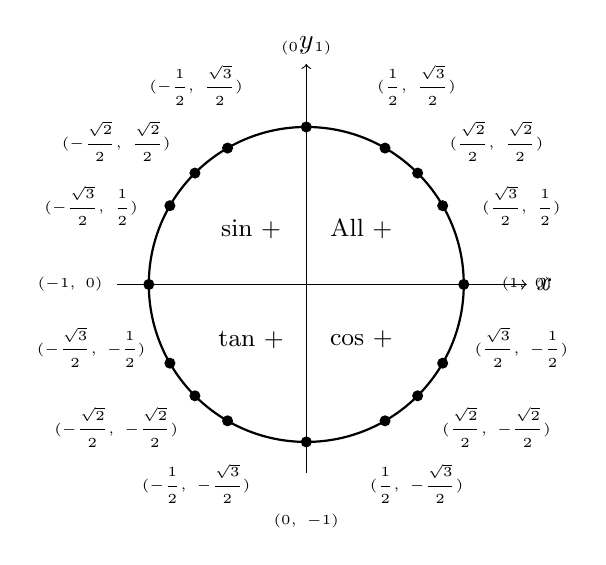
\begin{tikzpicture}[scale=2]
    % Draw the unit circle
    \draw[thick] (0,0) circle (1cm);
    % Axes
    \draw[->] (-1.2,0) -- (1.4,0);
    \draw[->] (0,-1.2) -- (0,1.4);
    % x and y labels adjusted
    \node[right] at (1.4,0) {$x$};
    \node[above] at (0,1.4) {$y$};
    % Points at common angles with labels
    \foreach \a/\d/\cs/\sn/\dx/\dy in {
        0/0^\circ/1/0/0.4/0.0,
        30/30^\circ/\dfrac{\sqrt{3}}{2}/\dfrac{1}{2}/0.5/0,
        45/45^\circ/\dfrac{\sqrt{2}}{2}/\dfrac{\sqrt{2}}{2}/0.5/0.2,
        60/60^\circ/\dfrac{1}{2}/\dfrac{\sqrt{3}}{2}/0.2/0.4,
        90/90^\circ/0/1/0.0/0.5,
        120/120^\circ/-\dfrac{1}{2}/\dfrac{\sqrt{3}}{2}/-0.2/0.4,
        135/135^\circ/-\dfrac{\sqrt{2}}{2}/\dfrac{\sqrt{2}}{2}/-0.5/0.2,
        150/150^\circ/-\dfrac{\sqrt{3}}{2}/\dfrac{1}{2}/-0.5/0,
        180/180^\circ/-1/0/-0.5/0.0,
        210/210^\circ/-\dfrac{\sqrt{3}}{2}/-\dfrac{1}{2}/-0.5/0.1,
        225/225^\circ/-\dfrac{\sqrt{2}}{2}/-\dfrac{\sqrt{2}}{2}/-0.5/-0.2,
        240/240^\circ/-\dfrac{1}{2}/-\dfrac{\sqrt{3}}{2}/-0.2/-0.4,
        270/270^\circ/0/-1/0.0/-0.5,
        300/300^\circ/\dfrac{1}{2}/-\dfrac{\sqrt{3}}{2}/0.2/-0.4,
        315/315^\circ/\dfrac{\sqrt{2}}{2}/-\dfrac{\sqrt{2}}{2}/0.5/-0.2,
        330/330^\circ/\dfrac{\sqrt{3}}{2}/-\dfrac{1}{2}/0.5/0.1
    } {
        % Calculate coordinates
        \coordinate (P) at ({cos(\a)},{sin(\a)});
        % Draw point
        \fill (P) circle (1pt);
        % Label coordinates
        \node[font=\tiny, anchor=center] at ($(P)+(\dx,\dy)$) {$(\cs,\ \sn)$};
    }
    % Quadrants
    \node at (0.35,0.35) {\small All $+$};
    \node at (-0.35,0.35) {\small $\sin$ $+$};
    \node at (-0.35,-0.35) {\small $\tan$ $+$};
    \node at (0.35,-0.35) {\small $\cos$ $+$};
\end{tikzpicture}
\end{center}
The cosine is the x-value, the sine is the y-value.

\subsection*{Radians and Degrees}
\[
180^\circ = \pi \text{ radians}, \quad 1^\circ = \dfrac{\pi}{180} \text{ radians}
\]
\textbf{Example:} Convert \( 135^\circ \) to radians:
\[
135^\circ \times \dfrac{\pi}{180^\circ} = \dfrac{3\pi}{4}
\]

\subsection*{Alternate Formulation}
For common angles, sine and cosine values can be calculated as:
\[
\sin \theta = \dfrac{\sqrt{n}}{2}, \quad \cos \theta = \dfrac{\sqrt{4 - n}}{2}
\]
where \( n \) corresponds to the following angles:
\begin{center}
\begin{tabular}{ll}
\( n = 0 \) & for \( \theta = 0^\circ \), \\
\( n = 1 \) & for \( \theta = 30^\circ \), \\
\( n = 2 \) & for \( \theta = 45^\circ \), \\
\( n = 3 \) & for \( \theta = 60^\circ \), \\
\( n = 4 \) & for \( \theta = 90^\circ \). \\
\end{tabular}
\end{center}

\subsection*{Reference Angles on the Unit Circle}
To find the trigonometric functions of any angle, find its reference angle and determine the sign based on the quadrant.

\textbf{Example:} Find \(\tan 225^\circ\).
\[
\theta_{\text{ref}} = 225^\circ - 180^\circ = 45^\circ
\]
\[
\tan 225^\circ = \tan (180^\circ + 45^\circ) = \tan 45^\circ = 1
\]
Since \(225^\circ\) is in Quadrant III, \(\tan\) is positive.

\textbf{Example:} Find \(\sin 210^\circ\).
\[
\theta_{\text{ref}} = 210^\circ - 180^\circ = 30^\circ
\]
\[
\sin 210^\circ = -\sin 30^\circ = -\dfrac{1}{2}
\]
Since \(210^\circ\) is in Quadrant III, \(\sin\) is negative.

\textbf{Example:} Find \(\cos 300^\circ\).
\[
\theta_{\text{ref}} = 360^\circ - 300^\circ = 60^\circ
\]
\[
\cos 300^\circ = \cos (360^\circ - 60^\circ) = \cos 60^\circ = \dfrac{1}{2}
\]
Since \(300^\circ\) is in Quadrant IV, \(\cos\) is positive.

\subsection*{Coterminal Angles}
Angles that differ by full rotations (\(360^\circ\)) are coterminal.

\textbf{Example:} \( \theta = -30^\circ \) is coterminal with \( 330^\circ \) because:
\[
-30^\circ + 360^\circ = 330^\circ
\]

\end{multicols}

\end{document}
